\documentclass[a4paper,10.5pt]{report}
\usepackage[top=2.5cm,bottom=3cm,right=3cm,left=3cm]{geometry}
\usepackage[utf8]{inputenc}
\usepackage[T1]{fontenc}
\usepackage[english]{babel}
\usepackage{graphicx,graphics,textcomp,setspace,lettrine}
\usepackage{amsmath,amssymb,amsfonts,indentfirst}
\usepackage[toc,page]{appendix} 
\usepackage{float}
\usepackage{array}
\usepackage{comment}
\usepackage{xcolor}
\usepackage{listings}
\usepackage{blindtext}
\usepackage{titling}
\usepackage{multicol}
\usepackage{enumitem}
\usepackage{ulem}
\usepackage{cancel}
\usepackage{wasysym}
\usepackage{hyperref}

\graphicspath{{plot/}}

\newcommand{\cfbox}[2]{%
    \colorlet{currentcolor}{.}%
    {\color{#1}%
    \fbox{\color{currentcolor}#2}}%
}

\usepackage[english, status=draft]{fixme}
\fxusetheme{color}

\lstset{numbers=left,
numberstyle=\tiny \bf ,
stepnumber=1,
numbersep=10pt,
firstnumber=1,
numberfirstline=true}

\lstset{frame=TBlr,
rulesepcolor=\color{black}}

\DeclareMathOperator{\e}{e}

\usepackage{fancyhdr}
\pagestyle{fancy}

\renewcommand{\headrulewidth}{1pt}
\fancyhead[L]{\leftmark}
\fancyhead[R]{}

\renewcommand{\footrulewidth}{1pt}
\fancyfoot[C]{\textbf{\thepage}} 
\fancyfoot[L]{}

\title{{\textsc{\Large{TP General Physics / M1}\\ [3cm]
      \textbf{\LARGE{High Velocity Cloud Analysis \\ in \\ HI4PI Data}}}} \\[2cm]}
\vfill
 \author{Antoine Marchal \\ [1cm]
Université Paris-Sud \\ 
Institut d’Astrophysique Spatiale \\
2016-2017}
\date{}


\begin{document}
\begin{titlingpage}
\maketitle
\end{titlingpage}
%% \tableofcontents
\newpage

\newpage
\chapter{Introduction}
The study of our own galaxy (the Milky Way) is especially complex by the fact that we are located inside. The sun is approximatly
at 8.5 kpc from the galactic center (noted G) and have a radial velocity due to the rotation around G of $ 220 \, km.s^{-1}$. 
As a fist approximation, we can discribe the galactic plane as a sum of three components : Gas (HI, neutral hydrogen), Star 
and Dark Matter. All around the galactic plane are located an important gas reservoir called the Milky Way Halo. To better 
understand how this reservoir constraint the physics of our galaxy, we must study it in detail. \\

\begin{figure}[h!]
  \centering
  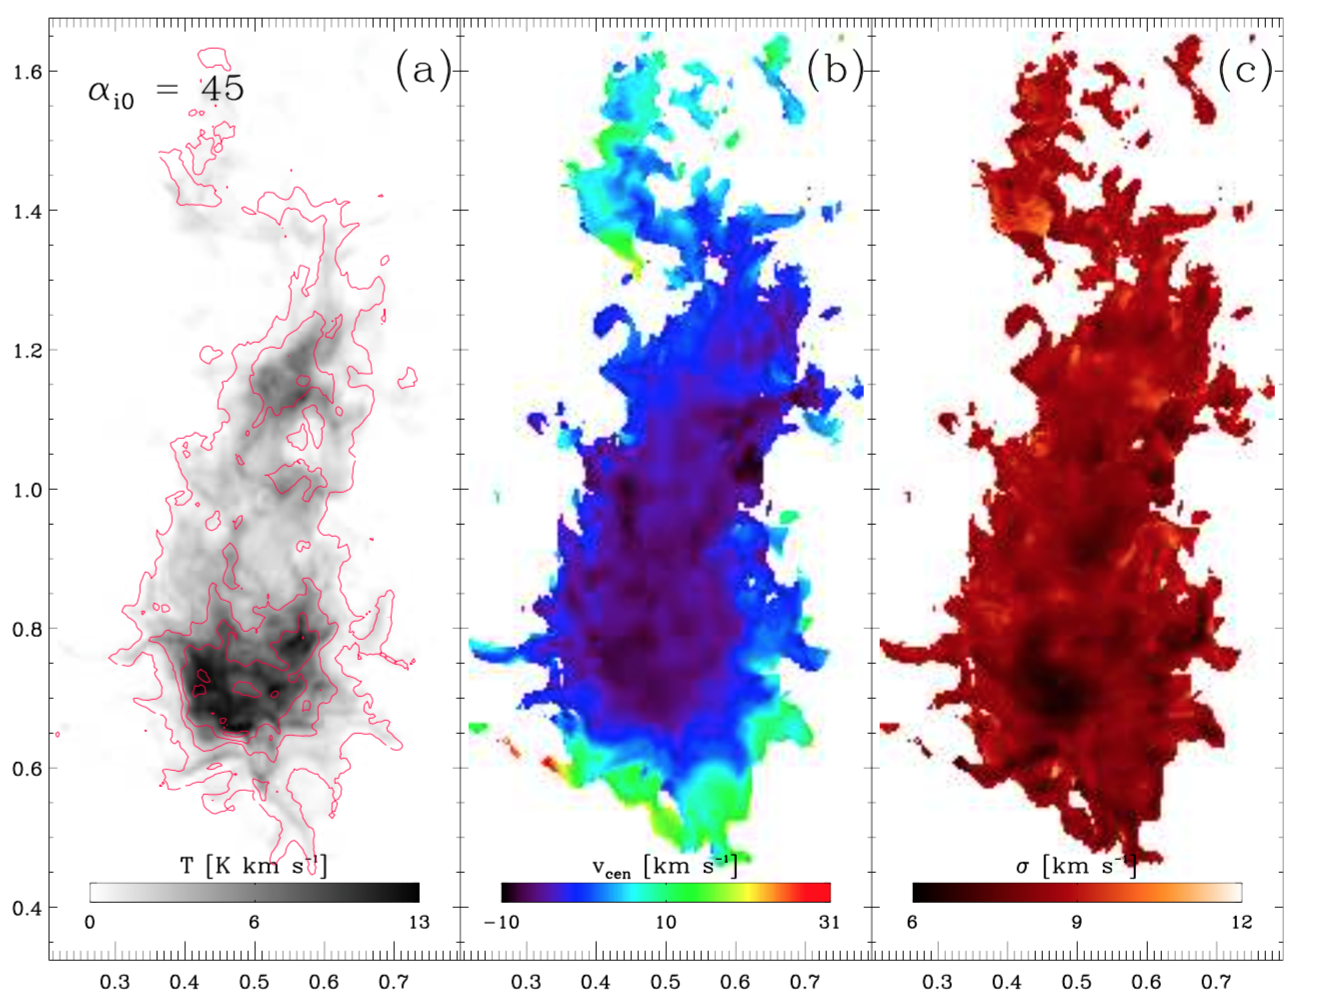
\includegraphics[width=4.in]{simulation}
  \label{fig::simulation}
  \caption{(a) Integrated intensity, (b) centroid velocity, and (c) velocity dispersion of a model CHVC (model Wb1a15b of 
    Heitsch & Putman (2009)), traveling at 45◦ to the observer. Contours are given at [1, 5, 9, 13] K km s−1.  / 
    (from Heitsch et al, 2016)}
\end{figure} \\
 
Since their discorevy by Muller et al (1963), High Velocity Clouds are studied as isolated objects. They are defined 
as neutral atomic hydrogen with radial velocity (typically $ V_r \approx 200 \, km.s^{-1}$) that cannot be explained by the rotation 
of the Milky Way (Wakker 1991). We present figure~\ref{fig::simulation} an HVC view from numerical simulation. 
The neutral hydrogen is very well observed since many years through the 21cm hyperfine structure line, and the latest full sky survey 
is the result of the HI4PI collaboration. More details are present in the recent article (in free access) : 
\color{blue} \url{https://arxiv.org/abs/1610.06175} \color{black}. 
This work is based on a single HVC cloud name HVC125+41-207 present in HI4PI. From the original data release, we develop a simple
method to obtain some approximations of the physical properties of this cloud and its environment. \\

\newpage 
\noindent
\underline{Physical constants} : \\
\begin{itemize}
\item[$\bullet$] Atomic mass of hydrogen : $m_H = 1.6737236 \times 10^{-27} \, kg$ 
\item[$\bullet$] Definition of a parsec : $pc = 3.085677581467192 \times 10^{16} \, m$
\item[$\bullet$] Mass of the Sun : $M_{\astrosun} = 1.9891 \times 10^{30} \, kg$
\item[$\bullet$] Mean mass per particle within the sphere : $\mu \approx 1.25 \, m_H$
\item[$\bullet$] Boltzmann constant : $k = 1.38064852 \times 10^{-23} \, m^2.kg.s^{-2}.K^{-1}$ 
\end{itemize} \\

%% \addcontentsline{toc}{chapter}{Introduction}
\chapter{Manipulation of hyperspectral data}
\section{Reading Data from HDF5 Files}
This work is based on Hyperspectral imaging (see representation figure~\ref{fig::hyperspectral}). 
For each pixel of the projected plan of sky we have an associated spectrum. \\

\begin{figure}[h!]
  \centering
  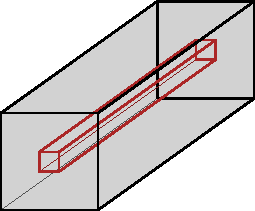
\includegraphics[width=3.in]{hyperspectral.pdf}
  \label{fig::hyperspectral}
  \caption{3D representation of a hyperspectral cube. All the points on a straight line in this cube compose a spectrum.
  We can select a sub-regoin of this cube which corresponds to a smaller part of the sky.}
\end{figure} \\

We propose to read the hyperspectral data which are formatted in a HDF5 file using the python langague.
A good documentation is available on the following link: 
\color{blue} \url{https://www.getdatajoy.com/learn/Read_and_Write_HDF5_from_Python} \color{black}

\section{High Velocity Cloud research}
The HVC HVC125+41-207 is located in the following spectral range : $v_{rad} (km.s^{-1}) = [-225, -185]$. 
From the article describing the HI4PI survey, we can clean the cube considering the rms value. For exemple we keep 
all values greater than $3 \times \sigma_{rms}$, with $\sigma_{rms}$ the sensitivity of HI4PI.
After selecting the spectral range, we can plot the HVC using the 'imshow' function in the matplotlib library 
(see \color{blue} \url{http://matplotlib.org} \color{black}) \\

Note that the galactic longitude range and the galactic latitude range of the cube are respectively
$l(deg) \in [119, 141]$ and $b(deg) \in [19, 51]$.

\begin{figure}[h!]
  \centering
  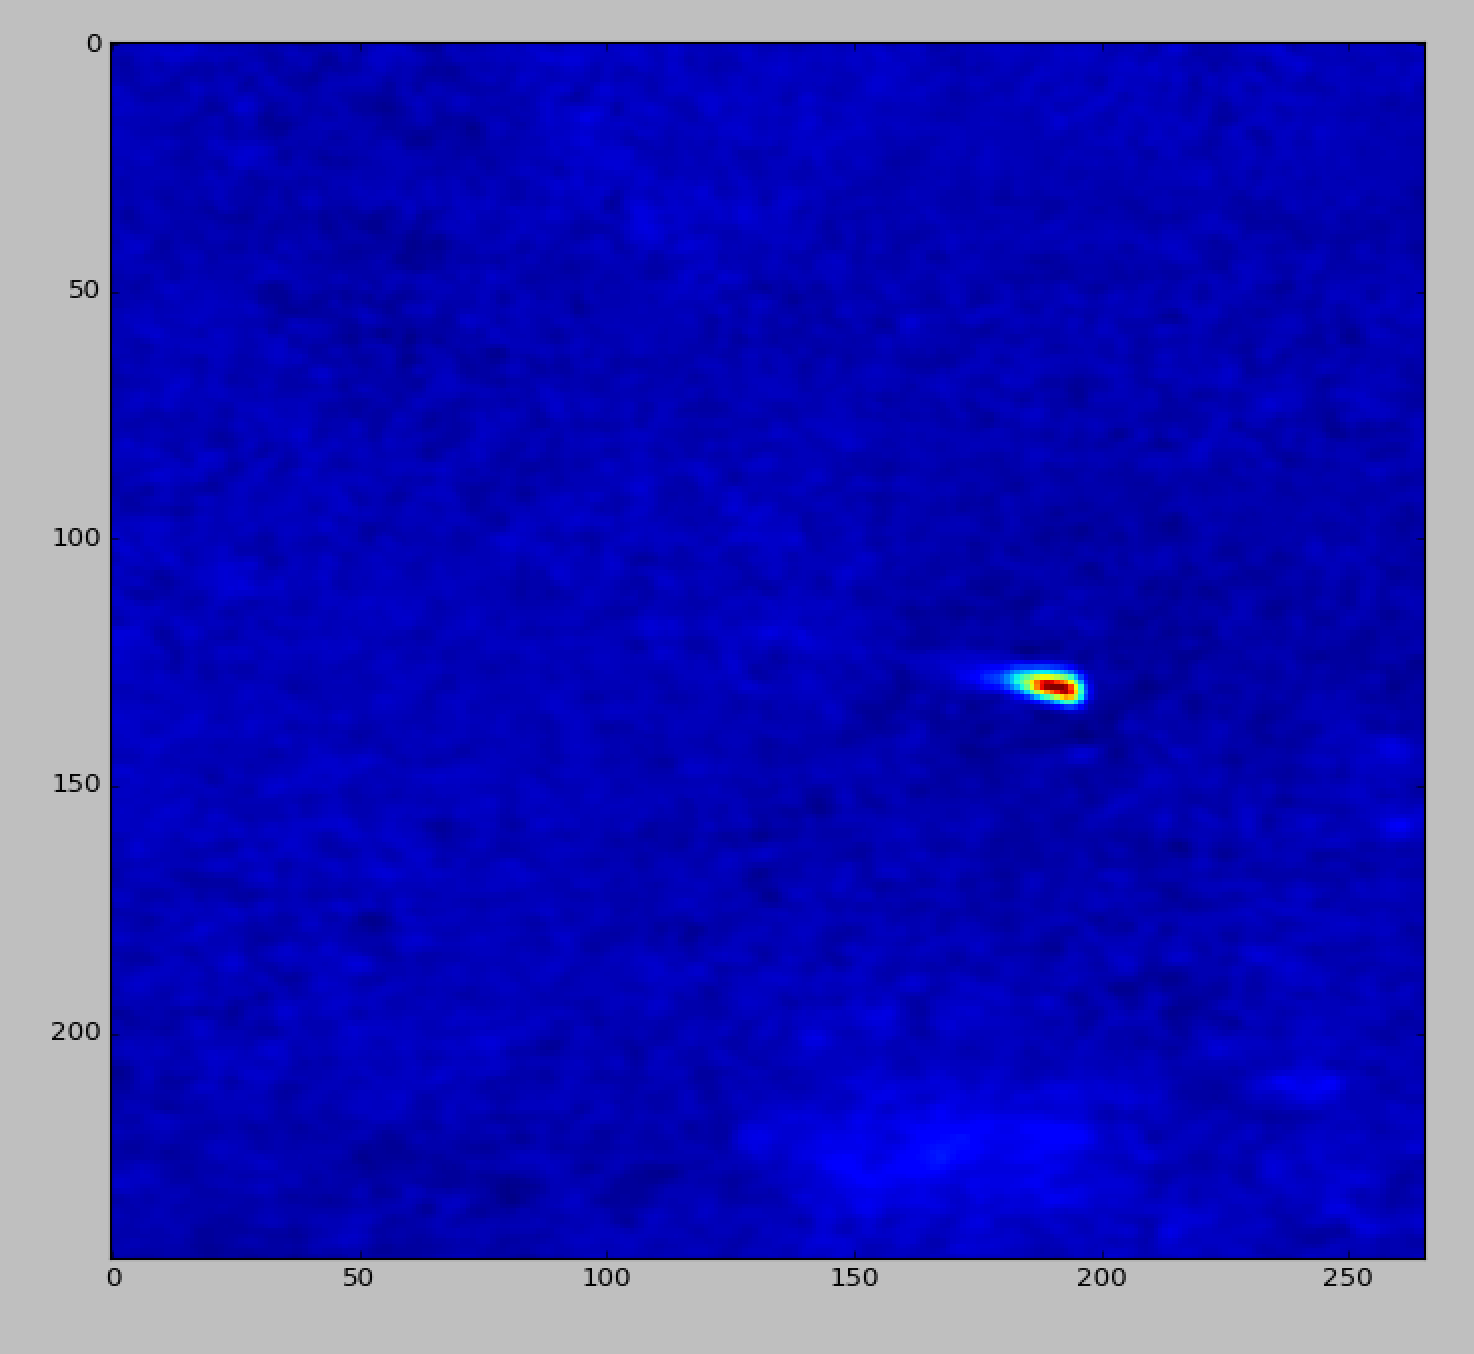
\includegraphics[width=4.in]{hvc.png}
  \label{fig::hvc}
  \caption{Representation of the HVC125+41-207 High Velocity Cloud}
\end{figure} \\

\chapter{Physical properties of the HVC}
\section{Mean spectra of the HVC}
To obtain some physical properties of this clump, we can analize the mean spectrum of the data.
We graphically represent the numerical calculation of the passage of hyperspectral data to the mean spectrum of the cloud
figure~\ref{fig::spectra}.

\begin{figure}[h!]
  \centering
  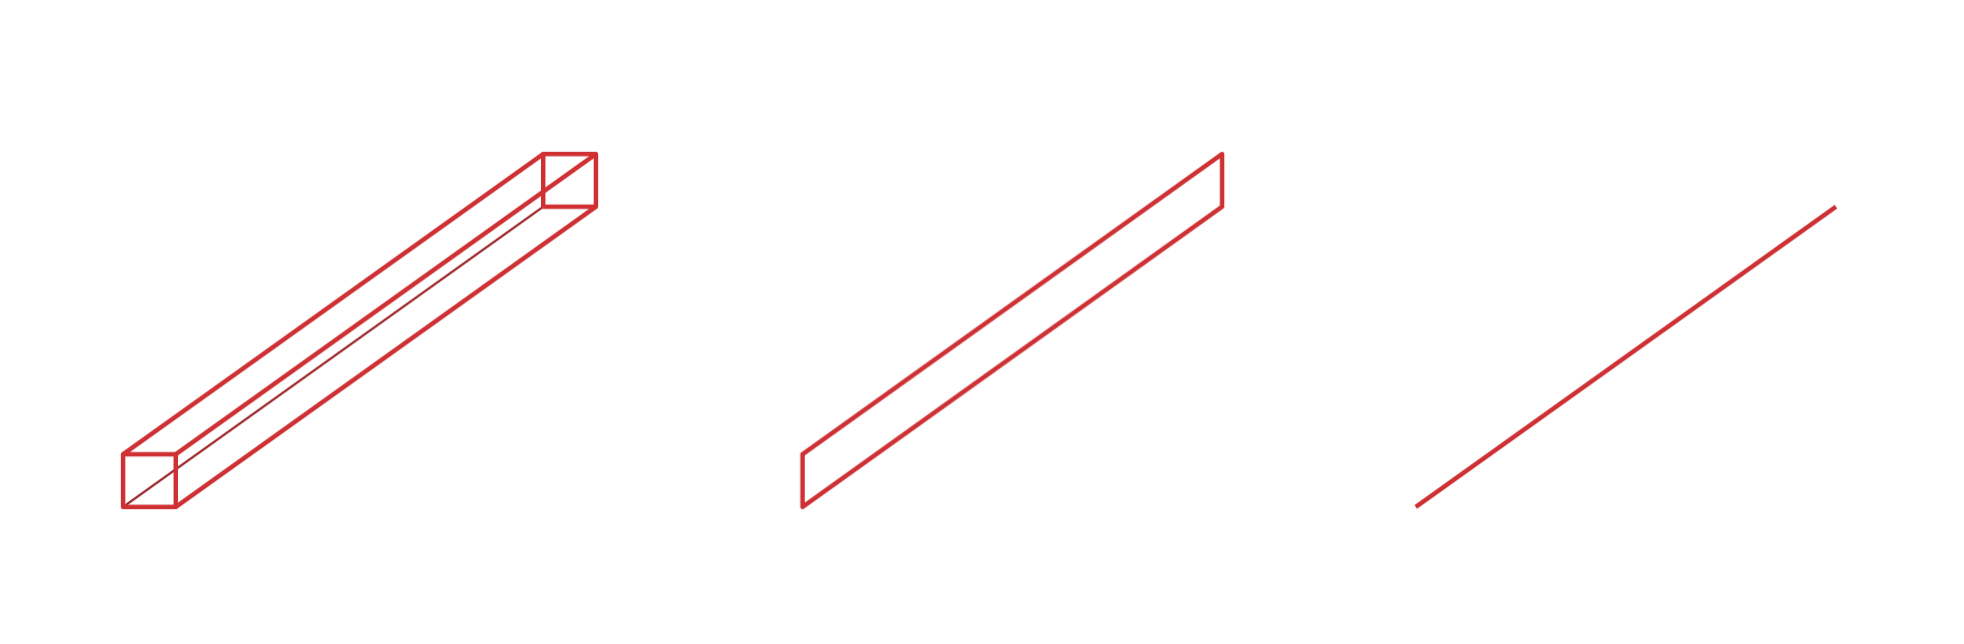
\includegraphics[width=6.in]{spectra.png}
  \label{fig::spectra}
  \caption{Representation of the passage of hyperspectral data to the mean spectrum of the cloud}
\end{figure} \\

\section{Spectral analysis}
As a first approximation, we can applied the Virial equilibrium to obtain the pressure outside the HVC as a function
of the distance d (preferentialy expressed in kpc which is a unit of length used in astronomy and astrophysics). 
This is actually nothing more than the pressure equilibrium between the inside medium and the outside medium.

\begin{align}
  \frac{P_s}{k} = \underbrace{\frac{\left< N_{HI} \right> \, T_k}{d \, \theta}}_\text{kinetic pressure} \,  
  \underbrace{- \, \frac{\mu^2 \, G \, \pi \, \left< N_{HI} \right>^2}{15 \, k}}_\text{gravitational pressure}
\end{align}  \\
where $\theta$ is the observed angular diameter in radian, $T_k$ is the kinetic temperature of the gas, d is the distance of the clump, 
$G$ and $k$ and respectively the gravitational constant and the Boltzmann constant, $\left< N_{HI} \right>$ is the mean value 
of the column density and $\mu$ the mean mass per particle within the sphere. \\

Tools to calculate the quantities that we have to get to compute the pressure as function of the distance of the cloud : \\

\noindent From the mean sprectra of the clump, we estimate $\left< N_{HI} \right>$ from 21 cm measurements. \\
\begin{align}
  \frac{\left< N_{HI} \right>}{cm^{-2}} = 1.82243 \times 10^{18} \times \int_{-\infty}^{+\infty} \left( \frac{T_b(v)}{K} \right) d\left( \frac{v}{km.s^{-1}}\right)
\end{align} 
where $T_b$ is the mean brightness temperature and $v$ is the the radial velocity. \\

\noindent Note that we can direclty get the surface density :
\begin{align}
  \Sigma = \frac{\left<N_{HI}\right> \, m_H \, pc^2}{M_\astrosun}
\end{align} \\
where $m_H$ is the atomic mass of hydrogen, $pc$ is the definition of a parsec,
and $M_{\astrosun}$ is the mass of the Sun. \\

If we consider that the temperature of our system is only due to the kinetic temperature (without turbulence for exemple), 
$T_k$ can be written as : 
\begin{align}
  T_k = \frac{m_H \, \sigma_v^2}{k} \, (K)
\end{align}
$\sigma_v$ is obtained by fitting a gaussian function on the mean spectra that we calculated previously.

\newpage
%\listoffixmes
\end{document}

